\documentclass[journal]{./IEEE/IEEEtran}
\usepackage{cite,graphicx}

\newcommand{\SPTITLE}{Sentence Generation Using User-Defined Predictive Text}
\newcommand{\ADVISEE}{John Alvin L. Sayson}
\newcommand{\ADVISER}{Fermin Roberto G. Lapitan}

\newcommand{\BSCS}{Bachelor of Science in Computer Science}
\newcommand{\ICS}{Institute of Computer Science}
\newcommand{\UPLB}{University of the Philippines Los Ba\~{n}os}
\newcommand{\REMARK}{\thanks{Presented to the Faculty of the \ICS, \UPLB\
                             in partial fulfillment of the requirements
                             for the Degree of \BSCS}}
        
\markboth{CMSC 190 Special Problem, \ICS}{}
\title{\SPTITLE}
\author{\ADVISEE
\REMARK
}
\pubid{\copyright~2018~ICS \UPLB}

%%%%%%%%%%%%%%%%%%%%%%%%%%%%%%%%%%%%%%%%%%%%%%%%%%%%%%%%%%%%%%%%%%%%%%%%%%

\begin{document}

% TITLE
\maketitle

% INTRODUCTION
\section{Introduction}
Since its conception, literature has served as the backbone of human history, documenting various events that transpired in the past. Throughout the years, however, literature became a creative outlet, bringing forth various books and stories that defined multiple generations.

It has always been humans that pioneered in creative writing, but in recent years it has become possible for artificial intelligence to write stories of their own, with information obtained from human sources.

Various website applications like AIWriter\cite{AIWriter} and Botnik's Voicebox\cite{Voicebox} help users write stories wherein source texts are processed to provide new outputs. AIWriter's process is fully automatic, instantly generating works depending on settings provided by the user in the beginning. On the other hand, Voicebox is more of a hands-on process as the user selects the words suggested by the application in writing their literary works. The suggested words are determined by the source text the user selected in the beginning, ranging from Harry Potter narrations to pancake recipes. If the selection range does not interest the user, they can provide their own source texts by uploading it to the website.

Both website applications improve writing time by doing away with manual word-for-word typing, providing either words or complete paragraphs for the users to use right away. This study intends to provide a similar convenience.

%writing time...
%cite Text prediction systems: a survey here.
Writing or typing time varies from person to person. For those with cognitive, perceptive, and/or physical disabilities, predictive text systems were their preferred medium in being able to communicate easier in social settings. \cite{GV2006} Being able to just use one tap to select words rather than multiple taps per letter, it allows for a great increase in convenience in conversation. Predictive text systems are now embedded in various native keyboards in mobile phones, wherein continuous usage can further personalize the suggested words to the user. Through this, the rate of communication between people can improve. This application aims to achieve a similar goal to that of the common predictive text system, but for more long-form outputs rather than short text messages. By providing an interface wherein users are given suggestions while in the middle of creating a piece, they can formulate ideas and receive new ones quicker than in a traditional writing application.

A notable difference from the proposed application from the aforementioned Voicebox is the introduction of genre selection, which eliminates the limit of sticking only to one source material at a time. The mixture of genres produce more varied outputs, and at the same time, more inventive story concepts. 

This paper shall discuss the proposed predictive text application in detail, as well as its intended implementation.

% OBJECTIVES
\section{Objectives}

\subsection{General Objective}
%The study aims to create an application wherein users can create various written works by selecting words provided by a predictive text interface.
The study aims to improve user writing speeds by allowing them to create long-form outputs using a predictive text system embedded in a text editor application.

\subsection{Specific Objectives}
\begin{enumerate}{\setlabelwidth{1.}}

\item[1.] Categorize input source material into genres and convert it into an interpretable representation;

\item[2.] Use a word-level language model to assess word relation in the sources provided;

\item[3.] Present word relation to the end user in the form of a predictive text writer interface;

\item[4.] Allow user text selection to influence future predictive outputs shown in the interface; and

\item[5.] Assess user experience and program outputs using surveys.

%\item[1.]Parse works by genre to create a network

%\item[2.]Use a model that can effectively assess word relation based from the datasets provided.

%\item[3.]Allow an end user to enter varied amounts of keywords for the writer to base outputs from.

%\item[4.]Parse the provided keyword inputs to influence the literary work output.

%\item[5.]Evaluate the readability and relevance of the output produced to what is asked through surveys.

%\item[6.]Objective 6

\end{enumerate}

% RRL
\section{Review of Related Literature}

%\subsection{Previous UPLB and Non-UPLB Works on NLG}

%\subsection{Concept Study of NLG}

%\subsection{Expected Content of RRL}
%\begin{enumerate}{\setlabelwidth{1.}}

%\item[1.]3 Papers Studying Concepts Related to NLG

%\item[2.]7 Papers on Related Studies (UPLB and non-UPLB)

%\item[3.]Applications of Methodologies (based on nos. 1 and 2)

%\end{enumerate}

%ACTUAL CONTENT OF RRL
To understand the possible applications and previous implementations of story and text generation, previous works in the field shall be observed.

%\subsection{Previous Advances in Text and Literary Work Generation}
%Online Works
%Text Generation from Keywords
Uchimoto, et al. presented various text-generation models in their paper wherein Japanese sentences are formed by feeding the program keywords which serve as the subjects of the sentence it produces. \cite{UKIHSS2002} 
%Discuss some of the language models...

A table of input-output pairs were provided by the authors, with inputs being words in groups of threes and the outputs being complete sentences. From this, a possible limitation provided by their application was that it could only accept three inputs at a time.

The authors have mentioned that the program was created for speakers that are not as fluent in Japanese be able to express sentences that they intend to speak but only know the main words that they want to express. This shows that text generation is not limited to recreational applications, and can be used for accessibility and elaboration. %continue...

\pubidadjcol
%Chinese Poetry Generation with Recurrent Neural Networks
X. Zhang and M. Lapata utilized recurrent neural networks in 2014 to generate Chinese poetry, which follows a specific format for it to be considered one.
\cite{ZXLM2014}
The Chinese poems that they generated follow the quatrain format, wherein four lines of poetry must have five or seven characters each.
The poetry generator functions similarly to Uchimoto's 2002 paper where keywords are accepted to outline the poem's main concept.
In creating the first line, a language model is used to rank candidates that satisfies criteria defined by the poetry format. Following lines are then based on the previous lines. This will ensure continuity from the first line to the last.

%Hierarchal Neural Story Generation
%A paper written by A. Fan, et al. in 2018 used generated sentence prompts that influences the resulting output.

Text generation has also ventured into literary fields with less constraints, specifically story writing.

In 2018, A. Fan, et al. added sentence prompt generation (aside from the expected story generation component) which was then based on to create the corresponding stories. \cite{FLD2018} These prompts are created using a convolutional language model, which contains a novel gated self-attention mechanism created by some of the authors. \cite{DFAG2016}
They also used a sequence-to-sequence network, a model that uses two recurrent neural networks as encoders and decoders, to generate the story based on the prompts trained on the convolutional language model. The sequence-to-sequence model depended upon the trained prompts from the convolutional language model, resulting in a fusion model, as referred to by the writers.

Results shown in the paper contained comparisons between the fusion model and another language model,  presenting the former's readability and higher quality of output over the latter. However, the authors mentioned that one of the limitations of the fusion model is the genericness of the prompts generated, compared to human prompts. This limits the results that can be generated as more specific and varied prompts can provide better results.

%THEORETICAL FRAMEWORK
%\section{Theoretical Framework}

% METHODOLOGY
\section {Methodology}
%\subsection{Expected Content of Methodology}
%\begin{enumerate}{\setlabelwidth{1.}}

%\item[1.]Model for the application

%\item[2.]Details about prototype (backend content)

%\item[3.]Initial results

%\end{enumerate}

%ACTUAL METHODOLOGY
This section shall contain the expected features of the implementation of the predictive text application, as well as the intended evaluation procedures that follow thereafter.

\subsection{Application Implementation}
The application shall be implemented using Python, as well as natural language processing libraries available in the programming language.

\subsection{Application Specifications}
\subsubsection{Input}
In preparation for user input, the application shall accept plaintext version of books. These shall then be converted into its bag-of-words equivalent. The new representation of the books shall be tagged with a genre defined by those entering the data.

\subsubsection{Processing}
After undergoing the selection of which sources to include, the predictive text application shall now generate a network of words. Words shall be connected in the network by their appearance after the previous node. 

%A graphical visualization is that these words are represented as a directed graph, where cycles may occur.

At this point, the application shall produce a list of starting words in the interface after the generation of the network. After the selection of the first word, a new list of selectable words shall replace the previous one, showing the words that have the highest probability of appearing after the previously selected word.

\subsubsection{Output}
Ending the writing process shall produce a tangible output for the user to review, allowing them to fine-tune their output as they wish.

\subsection{Application Evaluation}
The application is intended to target individuals with an interest in writing, therefore their experience in using the application is important in evaluating the resulting outputs. The evaluation shall be performed using a survey to assess the helpfulness and effectiveness of the application to their productivity in writing.

\subsection{Other Specifications}
As more and more input sources are uploaded in the application, the word network shall be able to accommodate the new data and update itself accordingly whenever the user selects the genres after uploading.

\section{Preliminary Results}
An initial version of the application was implemented, up to the ranking of the next possible word given one word. This version utilized the concept of Markov chains in computing various probabilities of the following words.

The text corpus was represented as a bag of words and a word-level Markov chain. Computations of probabilties were done using the following equation based on the Bayes' theorem, where A is the word to generate possible outputs from, and B is one of the candidate words:
$$ P(A \mid B) = \frac{P(B \mid A) \, P(A)}{P(B)} $$
%\begin{equation}

%\end{equation}

The multiple probabilities were stored in an adjacency list, of which the first value of the equation was pulled from. This is then multiplied to the probability of the A, computed by the following equation:
$$ P(A) = \frac{count(A)}{count(total)} $$

The product of the two are then divided by the probability of B, obtained the same way as A.

The computed values are then ranked and shown, the number of which depends on a parameter provided.

An example output is shown in Fig. 2, where the word to obtain possible candidates for the next words from is "harry".


\begin{figure}[!ht]
\begin{center}

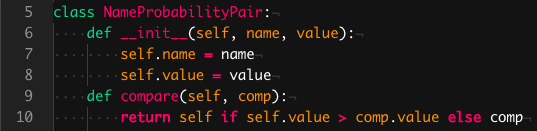
\includegraphics[width=90mm]{images/npp_initial.png}
\caption{A custom class named NameProbabilityPair, used in the comparison of the produced probabilities using Bayes' theorem.}

\end{center}
\end{figure}

\begin{figure}[!ht]
\begin{center}

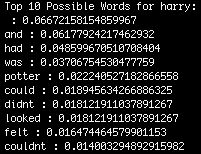
\includegraphics[height=50mm]{images/initial_output.png}
\caption{The output of the current version of the application.}

\end{center}
\end{figure}

%To be effective, the introduction should answer the questions ``Why and What For (Four)?" Expanded, these questions are:

%\subsection{Why is the topic of interest?}
%Start paragraph here...

%\subsection{What is the background on the previous solutions, if any?}

%\subsection{What is the background on potential solutions}

%\subsection{What was attempted in the present effor (research project)?}

%\subsection{What will be presented in this paper?}
%Subsection text here.

% MATERIALS AND METHODS
%\section{Materials and Methods}

%\subsubsection{First Heading}

%\subsubsection{Second Heading}

% RESULTS AND DISCUSSION
%\section{Results and Discussion}

% CONCLUSION AND FUTURE WORK
%\section{Conclusion and Future Work}

%assume that the user approves 
%filipino, bilingual support
%lesser suggestions compared to botnik
%10 suggestions or less

%find a justification, significance of the study
%why must it be predictive text?

%check botnik gallery

% BIBLIOGRAPHY
\bibliographystyle{./IEEE/IEEEtran}
\bibliography{./sayson-cs190-ieee}
\nocite{*}

% BIOGRAPHY
\begin{biography}
[{
\includegraphics{images/sayson.jpg}}]
{John Alvin L. Sayson} is an undergraduate student of the University of the Philippines Los Ba\~{n}os. Having an interest in writing and programming, he hopes to bridge the gap between the two through this study.
\end{biography}


\end{document}
 
